%%%%%%%%%%%%%%%%%%%%%%%%%%%%%%%%%%%%%%%%%%%%%%%%%%%%%%%%%%%%%%%%%%%%%%
% writeLaTeX Example: Academic Paper Template
%
% Source: http://www.writelatex.com
% 
% Feel free to distribute this example, but please keep the referral
% to writelatex.com
% 
%%%%%%%%%%%%%%%%%%%%%%%%%%%%%%%%%%%%%%%%%%%%%%%%%%%%%%%%%%%%%%%%%%%%%%
% How to use writeLaTeX: 
%
% You edit the source code here on the left, and the preview on the
% right shows you the result within a few seconds.
%
% Bookmark this page and share the URL with your co-authors. They can
% edit at the same time!
%
% You can upload figures, bibliographies, custom classes and
% styles using the files menu.
%
% If you're new to LaTeX, the wikibook is a great place to start:
% http://en.wikibooks.org/wiki/LaTeX
%
%%%%%%%%%%%%%%%%%%%%%%%%%%%%%%%%%%%%%%%%%%%%%%%%%%%%%%%%%%%%%%%%%%%%%%
\documentclass[twocolumn,showpacs,%
  nofootinbib,aps,superscriptaddress,%
  eqsecnum,prd,notitlepage,showkeys,10pt]{revtex4-1}

\usepackage[portuguese]{babel}
\usepackage[shortlabels]{enumitem}
\usepackage[utf8]{inputenc}
\usepackage{amssymb}
\usepackage{amsmath}
\usepackage{graphicx}
\usepackage{dcolumn}
\usepackage{xcolor}
\usepackage[pdfstartview=FitH,
            colorlinks,
            bookmarksnumbered,
            bookmarksopen,
            linktocpage,
            urlcolor=blue,
            linkcolor=red!70!black,
            citecolor=red!70!black]{hyperref}
\usepackage{float}
% \usepackage{multicol}
\usepackage{listings}
\usepackage{xfrac}
\usepackage{color}
\usepackage{tikz}
\usetikzlibrary{shapes, arrows}

\tikzstyle{terminator} = [rectangle, draw, text centered, rounded corners, minimum height=2em]
\tikzstyle{process} = [rectangle, draw, text centered, minimum height=2em]
\tikzstyle{decision} = [diamond, draw, text centered, minimum height=2em]
\tikzstyle{data}=[trapezium, draw, text centered, trapezium left angle=60, trapezium right angle=120, minimum height=2em]
\tikzstyle{connector} = [draw, -latex']

\definecolor{dkgreen}{rgb}{0,0.6,0}
\definecolor{gray}{rgb}{0.5,0.5,0.5}
\definecolor{mauve}{rgb}{0.58,0,0.82}

\lstset{frame=tb,
  language=[90]Fortran,
  aboveskip=3mm,
  belowskip=3mm,
  showstringspaces=false,
  columns=flexible,
  basicstyle={\small\ttfamily},
  numbers=none,
  numberstyle=\tiny\color{gray},
  keywordstyle=\color{blue},
  commentstyle=\color{dkgreen},
  stringstyle=\color{mauve},
  breaklines=true,
  breakatwhitespace=true,
  tabsize=4
}

\usepackage{booktabs}
\setlength{\heavyrulewidth}{1.5pt}
\setlength{\abovetopsep}{4pt}

\usepackage[nottoc,numbib]{tocbibind}
\usepackage{physics}

\usepackage[cmintegrals,cmbraces]{newtxmath}
\usepackage{ebgaramond-maths}

\newcommand{\C}{\mathbb{C}}
\newcommand{\R}{\mathbb{R}}
\newcommand{\N}{\mathbb{N}}
\newcommand{\Z}{\mathbb{Z}}

\DeclareMathOperator\erfc{erfc}
\newcommand*\diff{\mathop{}\!\mathrm{d}}
\newcommand*\Diff[1]{\mathop{}\!\mathrm{d^#1}}
\renewcommand{\leq}{\leqslant}
\renewcommand{\geq}{\geqslant}
\newcommand* \e{\mathrm{e}}

\makeatletter
  \DeclareSymbolFont{ntxletters}{OML}{ntxmi}{m}{it}
  \SetSymbolFont{ntxletters}{bold}{OML}{ntxmi}{b}{it}
  \re@DeclareMathSymbol{\leftharpoonup}{\mathrel}{ntxletters}{"28}
  \re@DeclareMathSymbol{\leftharpoondown}{\mathrel}{ntxletters}{"29}
  \re@DeclareMathSymbol{\rightharpoonup}{\mathrel}{ntxletters}{"2A}
  \re@DeclareMathSymbol{\rightharpoondown}{\mathrel}{ntxletters}{"2B}
  \re@DeclareMathSymbol{\triangleleft}{\mathbin}{ntxletters}{"2F}
  \re@DeclareMathSymbol{\triangleright}{\mathbin}{ntxletters}{"2E}
  \re@DeclareMathSymbol{\partial}{\mathord}{ntxletters}{"40}
  \re@DeclareMathSymbol{\flat}{\mathord}{ntxletters}{"5B}
  \re@DeclareMathSymbol{\natural}{\mathord}{ntxletters}{"5C}
  \re@DeclareMathSymbol{\star}{\mathbin}{ntxletters}{"3F}
  \re@DeclareMathSymbol{\smile}{\mathrel}{ntxletters}{"5E}
  \re@DeclareMathSymbol{\frown}{\mathrel}{ntxletters}{"5F}
  \re@DeclareMathSymbol{\sharp}{\mathord}{ntxletters}{"5D}
  \re@DeclareMathAccent{\vec}{\mathord}{ntxletters}{"7E}
\makeatother

\DeclareMathAlphabet\mathbfcal{OMS}{cmsy}{b}{n}

\begin{document}

\title{
Problemas de Sturm-Liouville unidimensionais: 
uma abordagem numérica usando o método do tiro
}
\author{Caio Tomás de Paula}
\affiliation{Departamento de Matemática, Universidade de Brasília, Brasil.}
%
\begin{abstract}
    Relatório entregue como parte do trabalho final do curso de Introdução a
    Métodos Computacionais em Equações Diferenciais Ordinárias (IMCEDO) do
    Programa de Pós-Graduação em Matemática (PPGMAT),
    ministrado pelo prof. Dr. Yuri Dumaresq Sobral no segundo semestre letivo
    de 2022 da Universidade de Brasília.
    O objetivo do trabalho foi resolver, numericamente, problemas de Sturm-Liouville,
    lançando mão do método do tiro. Dois problemas regulares e dois problemas singulares
    são resolvidos e a robustez do método é testada.
    Um dos problemas singulares trata de uma aplicação do método
    para resolver o problema de uma corda pendurada, investigado pela primeira vez por Daniel Bernoulli
    em 1732.
    Foi utilizada 
    \cite{Sturm-Liouville} como referência principal para o trabalho, além
    das notas de aula \cite{notas-aula-IMCEDO} e do livro \cite{iserles2008}.
\end{abstract}
%
\maketitle
%
\section{Introdução}
%
Em uma dimensão, o problema de Sturm-Liouville tem a forma geral
%
\begin{equation}
\label{eq:forma-geral-SL-1D}
    \left\{
    \begin{array}{l}
        -(p(x)y')' + q(x)y = \lambda r(x)y, \, a \leq x \leq b \\ 
        \alpha y(a) + \beta y'(a) = 0, \\ 
        \gamma y(b) + \delta y'(b) = 0.
    \end{array}
    \right.
\end{equation}
%
O valor de $\lambda$ não é especificado na equação: encontrar $\lambda$
tal que o problema admita solução não-trivial é parte do problema de Sturm-Liouville.
Tais valores de $\lambda$, quando existem, são chamados \textbf{autovalores}
do problema, e as soluções correspondentes são as \textbf{autofunções} associadas
a cada $\lambda$. Esta terminologia vem do fato de que as soluções correspondem
aos autovalores/autofunções de um operador diferencial definido num espaço
de funções com um produto interno apropriado. 

A teoria de Sturm-Liouville é muito importante, em particular, no contexto
da Matemática Aplicada: problemas de Sturm-Liouville aparecem com muita
frequência, em particular quando se lida com EDPs lineares separáveis.
Alguns exemplos são:
%
\begin{itemize}
    \item a equação do calor:
    %
    \[
        u_t = \kappa u_{xx}.
    \]
    %
    \item a equação da onda:
    %
    \[
        u_{tt} = c^2u_{xx}.
    \]
    %
    \item a equação de Poisson:
    %
    \[
        \laplacian u = f(x,y).
    \]
    %
    \item a equação de Laplace:
    %
    \[
        \laplacian u = 0.
    \]
    %
    % \item a equação de Helmholtz:
    % %
    % \[
    %     \laplacian u + \alpha^2u = 0, \, \alpha\in\R.
    % \]
    %
    \item a equação de Schrödinger unidimensional independente do tempo:
    %
    \[
        \hat{H} \phantom{i} |\Psi\rangle
        = E \phantom{i} |\Psi\rangle.
    \]
    %
\end{itemize}
%
Vamos começar considerando problemas \textbf{regulares}, que são da forma
\eqref{eq:forma-geral-SL-1D} e satisfazem as condições
%
\begin{enumerate}[(i)]
    \item $p, q > 0$ em $[a,b]$;
    \item $p, q, r\in C^1([a,b])$;
    \item $\alpha, \beta, \gamma, \delta \in\R$ com $|\alpha| + |\beta| > 0$
    e $|\gamma| + |\delta| > 0$.
\end{enumerate}
%
Ademais, para implementarmos o método do tiro vamos requerer que
%
\begin{itemize}
    \item[(iv)] $p, q, r\in C^2([a,b])$.
\end{itemize}
%
Ao final, vamos resolver um \textbf{problema singular} do primeiro tipo, que tem
a forma
%
\begin{equation}
\label{eq:forma-geral-SL-1D-singular1}
    \left\{
    \begin{array}{l}
        -(p(x)y')' + q(x)y = \lambda r(x)y, \, a < x < b \\ 
        |y(a)| < \infty \\ 
        \gamma y(b) + \delta y'(b) = 0, \, |\gamma| + |\delta| \neq 0.
    \end{array}
    \right.
\end{equation}
%
Neste caso, pediremos que
%
\begin{enumerate}[(i)]
    \item $p(x) \geq 0$ seja contínuo em $[a,b]$, diferenciável em $a$, não nulo em $(a,b]$
    e tal que $p(a) = 0$ e $p'(a) \neq 0$;
    \item $q\in C^1([a,b])$;
    \item $p,q$ funções reais e $\gamma, \delta\in\R$;
    \item $r\in C^1([a,b])$ e ou $r(x) > 0$ em $[a,b]$ ou $r(x) = (x-a)^m\rho(x)$
    com $m>0$ e $\rho(x) > 0$ contínua em $[a,b]$.
\end{enumerate}
%
Para utilizar o método do tiro neste tipo de problema,
também vamos pedir que $p,q,r$ sejam de classe $C^2$
em $[a,b]$.

Em várias dimensões, o problema de autovalor assume a forma da
\textbf{equação de Helmholtz}, dada por
%
\begin{equation}
\label{eq:helmholtz}
    \left\{
    \begin{array}{l}
        \laplacian u + \alpha^2u = 0, \, \mathbf{x}\in\Omega \\ 
        F(u, u_{x_1}, u_{x_2}, \dots, u_{x_n}) = 0, \mathbf{x}\in\partial\Omega.
    \end{array}
    \right.
\end{equation}
%
O principal resultado da teoria de Sturm-Liouville afirma que
%
\begin{enumerate}
    \item os autovalores são reais e podem ser ordenados,
    %
    \[
        0 < \lambda_1 < \lambda_2 < \cdots < \lambda_n < \cdots \to \infty.
    \]
    %
    \item a cada autovalor $\lambda_n$ está associada uma única (a menos
    de multiplicação por escalar) autofunção $y_n$, que tem exatamente 
    $n-1$ zeros em $(a,b)$, chamada \textbf{$n$-ésima solução fundamental}.

    \item as autofunções (normalizadas) formam uma base ortonormal com
    respeito ao produto interno de peso $r$\footnote{A rigor, é necessário também que
    $y_n$ e $y_m$ sejam quadrado-integráveis em $[a,b]$ com respeito a $r$.},i.e.,
    %
    \[
        \left\langle y_n, y_m \right\rangle
        = \int_a^b y_n(x)y_m(x)r(x) \diff x
        = \delta_{mn},
    \]
    %
    sendo $\delta_{mn}$ o delta de Kronecker:
    %
    \[
        \delta_{mn} = \left\{
        \begin{array}{l}
            1, \, n = m \\
            0, \, n\neq m.
        \end{array}
        \right.
    \]
    %
\end{enumerate}
%
Para resolver este problema numericamente, vamos usar o
\textbf{método do tiro}.
%
\section{Resultados}
\label{sec:resultados}
%
\subsection{O método numérico}
%
A ideia do método do tiro é transformar a solução de um PVC na solução
de (alguns) PVIs combinada à solução de uma equação (ou sistema) algébrico,
dada pela solução do PVI.
Para ilustrar o funcionamento do método aplicado a este problema, considere
o problema de autovalor unidimensional com c.c.'s de Dirichlet:
%
\[
    \left\{
    \begin{array}{l}
        y'' + \lambda y = 0, \, a \leq x \leq b \\ 
        y(a) = 0 = y(b).
    \end{array}
    \right.
\]
%
Se $\lambda$ é um autovalor e $y(x) = y(x,\lambda)$ é a autofunção correspondente,
então $y'(a) \neq 0$ e, portanto, existe uma única autofunção normalizada com $y'(a) = 1$.
Esta autofunção normalizada deve satisfazer o PVI
%
\[
    \left\{
    \begin{array}{l}
        u'' + \lambda u = 0, \, a \leq x \leq b \\ 
        u(a) = 0, \, u'(a) = 1
    \end{array}
    \right.
\]
%
e, também, a equação $u(b) = u(b,\lambda) = 0$. Reciprocamente, se $u$ é solução
do PVI anterior e é tal que $u(b,\lambda) = 0$, então $\lambda$ é um autovalor
do problema de Sturm-Liouville e $y(x) = u(x,\lambda)$ é a autofunção normalizada correspondente.

De maneira geral, se temos o problema \eqref{eq:forma-geral-SL-1D}, então o PVI associado é
%
\begin{equation}
\label{eq:PVI-geral-tiro}
    \left\{
        \begin{array}{l}
            -(p(x)u')' + (q(x) - \lambda r(x))u = 0, \, a \leq x \leq b \\ 
            u(a) = -\beta/\sqrt{\alpha^2 + \beta^2}, \\ 
            u'(a) = \alpha/\sqrt{\alpha^2 + \beta^2}.
        \end{array}
    \right.
\end{equation}
%
Pela simplicidade dos autovalores e unicidade das autofunções,
segue que a única autofunção (normalizada) associada a cada autovalor é tal que
%
\[
    y(a) = -\beta/\sqrt{\alpha^2 + \beta^2}, \quad
    y'(a) = \alpha/\sqrt{\alpha^2 + \beta^2}.
\]
%
Assim, resolver o  PVC \eqref{eq:forma-geral-SL-1D}
é \textbf{equivalente} (tanto conceitual quanto numericamente)
a resolver o PVI \eqref{eq:PVI-geral-tiro}
e encontrar a raiz de $F(\lambda) = 0$, sendo
%
\begin{equation}
\label{eq:eq-algebrica-tiro}
    F(\lambda) = \gamma u(b, \lambda) + \delta u'(b, \lambda).
\end{equation}
%
Feito isto, a autofunção normalizada é $y(x) = u(x,\lambda)$.

Essencialmente, o algoritmo é:
%
\begin{enumerate}
    \item propor uma estimativa $\lambda_n^i$ para o autovalor $\lambda_n$; 
    \item resolver o PVI em $u(x, \lambda_n^i)$ dado por \eqref{eq:PVI-geral-tiro};
    \item avaliar o quão longe de $0$ está $F(\lambda_n^i)$:
    %
    \begin{enumerate}
        \item se muito longe, usamos um método iterativo para obter um próximo 
        chute $\lambda_n^{i+1}$ e voltamos ao passo 1;
        \item se perto o bastante, paramos: o autovalor foi encontrado;
    \end{enumerate}
    %
    \item encontrado o autovalor, resolvemos o PVI \eqref{eq:PVI-geral-tiro} uma
    última vez para determinar a autofunção associada.
\end{enumerate}
%
É possível mostrar (cf. \cite[p.~304-305, Teo.~186 - 188]{Sturm-Liouville}) que
podemos usar os métodos da bisseção e de Newton-Raphson para encontrar os autovalores
em problemas de Sturm-Liouville regulares\footnote{Os mesmos resultados valem, com as devidas
alterações nas demonstrações, para problemas de Sturm-Liouville singulares.}.

Utilizamos o método de Runge-Kutta explícito de 4ª ordem clássico (RKE$4$) dado pela
Tabela \ref{tab:RKE4} para resolver os PVIs e um método da bisseção para
avançar nas estimativas para os autovalores.
%
\begin{table}[H]
    \centering
    \caption{Tabela de Butcher do método de RK utilizado}
    \begin{tabular}{c|cccc}
        $0$ &  &  &  &  \\
        $\sfrac{1}{2}$ & $\sfrac{1}{2}$ &  &  &  \\
        $\sfrac{1}{2}$ & $0$ & $\sfrac{1}{2}$ &  &  \\
        $1$ & $0$ & $0$ & $1$ &  \\
        \hline
         & $\sfrac{1}{6}$ & $\sfrac{1}{3}$ & $\sfrac{1}{3}$ & $\sfrac{1}{6}$
    \end{tabular}
    \label{tab:RKE4}
\end{table}
%
A Figura \ref{fig:flux-codigo} ilustra, diagramaticamente, a maneira como
a lógica do código utilizado foi construída.
%
\begin{figure}[H]
    \centering
    \begin{tikzpicture}[node distance = 2cm]
        \node [terminator, fill=blue!20] (start) {\textbf{Inicialização das variáveis}};
        
        \node [process, fill=blue!20] at (0,-1.5) (PVI2) 
        {Resolver o PVI \eqref{eq:PVI-geral-tiro} para $\lambda = \lambda_n^i$};
        
        \node [decision, fill=blue!20, below of = PVI2] (decision) {$F(\lambda_n^i) < \mathrm{TOL}$?};
        
        \node [process, fill=red!20] at (3.7,-1.5) (chute) 
        {$\lambda_n^i \to \lambda_n^{i+1}$};
        
        \node [process, fill=green!20] at (0,-6) (encontrado)
        {Autovalor $\lambda_n$ encontrado!};
        
        \node [process, fill=blue!20] at (0,-7.5) (PVIFinal) 
        {Resolver o PVI \eqref{eq:PVI-geral-tiro} para $\lambda = \lambda_n$};

        \node [terminator, fill=teal!20] at (-3.7,-4.5) (metodo)
        {RKE$4$};
        
        \node [data, fill=blue!20] at (0,-9) (salvamento) 
        {Salvar solução};
        
        \node [terminator, fill=blue!20] at (0,-10.5) (end) {\textbf{Fim}};
        
        \node[draw=none] at (2.40, -3.25) (no) {Não};
        \node[draw=none] at (0.35, -5.20) (yes) {Sim};
        
        \path [connector] (start) -- (PVI2);
        \path [connector] (PVI2) -- (decision);
        \path [connector] (decision) -| (chute);
        \path [connector] (decision) -- (encontrado);
        \path [connector] (chute) -- (PVI2);
        \path [connector] (metodo) |- (PVI2);
        \path [connector] (metodo) |- (PVIFinal);
        \path [connector] (encontrado) -- (PVIFinal);
        \path [connector] (PVIFinal) -- (salvamento);
        \path [connector] (salvamento) -- (end);
    \end{tikzpicture}
    \caption{Fluxograma do código}
    \label{fig:flux-codigo}
\end{figure}
%
\subsection{Validação do método}\label{subsec:validacao}
%
Para testar e validar o método, resolvemos o problema de Sturm-Liouville
%
\begin{equation}
\label{eq:firstproblem}
    \left\{
        \begin{array}{l}
            y'' + \lambda y = 0, \, 0 \leq x \leq 1 \\ 
            y(0) = y(1) = 0,
        \end{array}
    \right.
\end{equation}
%
cujos autovalores e autofunções podem ser calculados sem dificuldades e são dados por
%
\[
    \lambda_n = n^2\pi^2, \quad y_n = \sin(n\pi x).
\]
%
Este problema aparece ao resolvermos a equação do calor em uma barra unidimensional
com ambas extremidades à temperatura constante e igual a $0$.

Resolvendo este PVC com chutes iniciais para a bisseção $[a,b] = [n^2\pi^2 -2, n^2\pi^2 + 5]$, 
encontramos as autofunções da Figura \ref{fig:first-problem}.
Traçamos as autofunções normalizadas $\sin(n\pi x)/\pi x$ na Figura \ref{fig:first-problem-check},
mostrando
que o método encontrou corretamente os autovalores e as autofunções.
%
\begin{figure}[H]
    \centering
    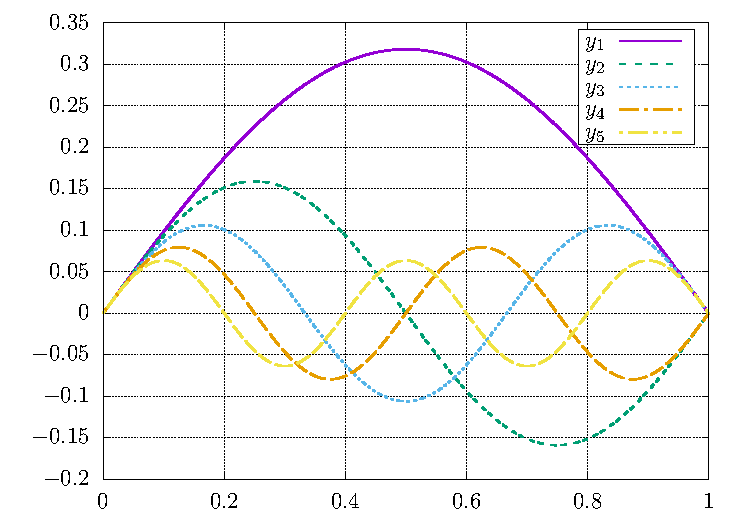
\includegraphics[width=.49\textwidth]{Relatório/Figuras/FirstProblem.pdf}
    \caption{Gráficos das primeiras cinco autofunções normalizadas
    encontradas numericamente.}\label{fig:first-problem}
\end{figure}
%
%
\begin{figure}[H]
    \centering
    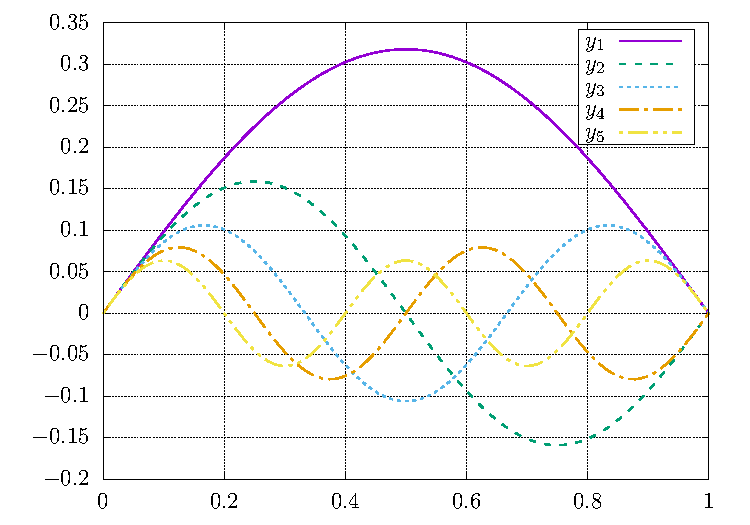
\includegraphics[width=.49\textwidth]{Relatório/Figuras/FirstProblem_check.pdf}
    \caption{Gráficos das primeiras 5 autofunções normalizadas.}\label{fig:first-problem-check}
\end{figure}
%
%
\subsection{Análise de robustez do método em relação ao intervalo inicial}\label{subsec:robustez}
%
Ainda com o problema \eqref{eq:firstproblem}, foi feita uma análise da robustez do método.
A Tabela \ref{tab:robustez} resume os resultados. Foram feitos alguns palpites de intervalos
iniciais para início da bisseção e percebe-se que o método divergiu apenas quando o intervalo
inicial não continha nenhum autovalor em seu interior, como esperado. Colocou-se $\infty$
para o número de iterações como ilustração dos casos divergentes, com os autovalores encontrados
em vermelho: o método da bisseção, de fato, convergiu, mas não para o local adequado e, por isso,
o número de iterações foi colocado como $\infty$, já que o método do tiro não parou de iterar.
%
\begin{table}[H]
    \centering
    \caption{Análise da robustez do método do tiro.}
    \begin{tabular}{cc|cc|c|c}
        % \hline
        \multicolumn{2}{c}{Intervalo inicial} & \multicolumn{2}{c}{Autovalor encontrado}
        & \multicolumn{2}{c}{} \\
        \hline
        $a$ & $b$ & $n$ & $\lambda_n$ & \# iterações & \% erro \\
        \hline
        $-10000$ & $1000$ & $3$ & $88.826439547119662$ & $35$ & $10^{-7}$ \\
        $-100$ & $1000$ & $9$ & $799.43796582520008$ & $28$ & $10^{-6}$ \\
        $-1$ & $2$ & --- & \textcolor{red}{$2$} & $\infty$ & --- \\
        $500$ & $30000$ & $54$ & $28780.159626156092$ & $27$ & $10^{-3}$ \\
        $1$ & $3$ & --- & \textcolor{red}{$3$} & $\infty$ & --- \\
        $1$ & $10$ & $1$ & $9.8696044087409973$ & $24$ & $10^{-7}$ \\
        $-1000$ & $10$ & $1$ & $9.8696043915697373$ & $35$ & $10^{-7}$ \\
        \hline
    \end{tabular}
    \label{tab:robustez}
\end{table}
%
Vemos, portanto, que o método do tiro utilizando o método da bisseção é robusto em relação
ao intervalo inicial, isto é, não precisamos escolher intervalos iniciais muito específicos
para que o método convirja.
Esta propriedade vem do fato de que se o intervalo inicial contém um autovalor, i.e., se
o intervalo inicial contém raiz de $F(\lambda)$, então a bisseção invariavelmente convergirá
para uma raiz.
%
\subsection{Resolvendo um problema regular com c.c.'s de Robin}\label{subsec:aplicacao}
%
Vamos considerar agora o PVC
%
\begin{equation}
\label{eq:secondproblem}
    \left\{
        \begin{array}{l}
            -y'' + xy = \lambda\cos(x)y, \, 0 \leq x \leq 1 \\ 
            y(0) + y'(0) = 0 \\ 
            y(1) + y'(1) = 0.
        \end{array}
    \right.
\end{equation}
%
Diferentemente do PVC \eqref{eq:firstproblem}, neste problema não sabemos, \textit{a priori},
quem são os autovalores e as autofunções\footnote{De fato, a solução da EDO deste PVC
é dada em termos das \href{https://en.wikipedia.org/wiki/Airy_function}{funções de Airy}
de primeira e segunda espécies.}.
Usando \eqref{eq:PVI-geral-tiro}, o PVI que precisamos resolver é
%
\[
    \left\{
        \begin{array}{l}
            -u'' + xu = \lambda \cos(x)u, \, 0 \leq x \leq 1 \\ 
            u(0) = -1/\sqrt{2} \\ 
            u'(0) = 1/\sqrt{2}.
        \end{array}
    \right.
\]
%
Aplicando o método do tiro, obtemos os resultados mostrados
na Tabela \ref{tab:secondproblem} e na Figura \ref{fig:second-problem}.
%
\begin{table}[H]
    \centering
    \caption{Intervalos iniciais e autovalores encontrados para o PVC \eqref{eq:secondproblem}.}
    \begin{tabular}{cc|cc|c}
        % \hline
        \multicolumn{2}{c}{Intervalo inicial} & \multicolumn{2}{c}{Autovalor encontrado} & \\
        \hline
        $a$ & $b$ & $n$ & $\lambda_n$ & \# iterações \\
        \hline
        $0$ & $15$ & $1$ & $13.57597859$ & $31$ \\
        $25$ & $60$ & $2$ & $49.200691955629736$ & $31$ \\
        $70$ & $120$ & $3$ & $108.32595458952710$ & $32$ \\
        $180$ & $240$ & $4$ & $191.05031406506896$ & $30$ \\
        $200$ & $350$ & $5$ & $297.39334740152117$ & $34$ \\
        \hline
    \end{tabular}
    \label{tab:secondproblem}
\end{table}
%
O gráfico mostra, em particular, que as autofunções oscilam com amplitudes
cada vez maiores.
%
\begin{figure}[H]
    \centering
    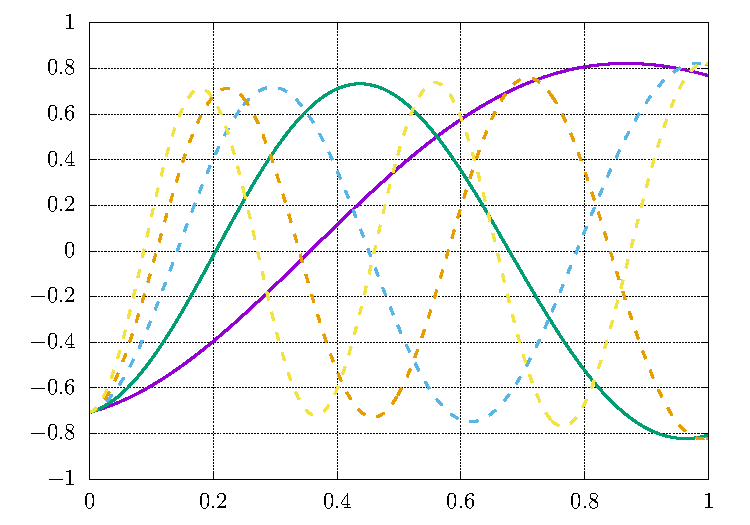
\includegraphics[width=.5\textwidth]{Relatório/Figuras/SecondProblem.pdf}
    \caption{Autofunções (normalizadas) para o problema de Sturm-Liouville
    \eqref{eq:secondproblem}.}
    \label{fig:second-problem}
\end{figure}
%
%
\subsection{Um pouco sobre problemas singulares}\label{subsec:singulares}
%
O método do tiro aplicado a problemas singulares do tipo \eqref{eq:forma-geral-SL-1D-singular1}
é levemente diferente. É possível mostrar \cite[Lema 148, p.~233]{Sturm-Liouville}
que se $y$ é solução deste tipo de problema,
então necessariamente
%
\[
   (q(a) - \lambda r(a))y(a) - p'(a)y'(a) = 0.
\]
%
Além disso, também é possível mostrar que soluções limitadas não-triviais deste tipo de
problema são tais que $y(a) \neq 0$. Portanto, normalizamos a autofunção exigindo que
%
\[
    y(a) = 1.
\]
%
Logo, uma autofunção (normalizada) satisfaz as condições iniciais
%
\[
    y(a) = 1, \quad
    y'(a) = \frac{q(a) - \lambda r(a)}{p'(a)},
\]
%
ou seja, o método do tiro, neste caso, se resume em resolver o PVI
%
\begin{equation}
\label{eq:algebrica-tiro-singular}
    \left\{
        \begin{array}{l}
            -(p(x)u')' + (q(x) - \lambda r(x))u = 0, \, a \leq x\leq b \\ 
            u(a) = 1, \\ 
            u'(a) = (q(a) - \lambda r(a))/p'(a)
        \end{array}
    \right.
\end{equation}
%
e encontrar a raiz de
%
\[
    F(\lambda) = \gamma u(b,\lambda) + \delta u'(b, \lambda).
\]
%
Aplicamos este método para resolver o PVC
%
\begin{equation}
\label{eq:singproblem}
    \left\{
        \begin{array}{l}
            -(xy')' = \lambda xy, \, 0 \leq x\leq 1 \\ 
            |y(0)| < \infty, \\ 
            \gamma y(1) + \delta y'(1) = 0,
        \end{array}
    \right.
\end{equation}
%
que aparece quando resolvemos, por exemplo, a equação do calor numa placa circular
cujas faces estão isoladas e cuja circunferência obedece à Lei de Newton do resfriamento.
Sua EDO nada mais é do que a equação de Bessel de ordem $0$ e parâmetro $\lambda$, de modo
que as autofunções são dadas em termos da função de Bessel de primeira espécie de ordem $0$:
%
\[
    y_n(x) = J_0\left(\sqrt{\lambda_n}x\right), \, n = 1, 2, \dots,
\]
%
com $\lambda_n$ raízes de
%
\[
    F(\lambda) = J_0\left(\sqrt{\lambda}\right) + \sqrt{\lambda}J_0'\left(\sqrt{\lambda}\right)
               = J_0\left(\sqrt{\lambda}\right) - \sqrt{\lambda}J_1\left(\sqrt{\lambda}\right).
\]
%
O PVI associado para o método do tiro é, portanto,
%
\[
    \left\{
        \begin{array}{l}
            -(xu')' = \lambda xu, \, 0 \leq x\leq 1 \\ 
            u(a) = 1, \, u'(a) = 0.
        \end{array}
    \right.
\]
%
Resolvendo-o, obtemos os autovalores na Tabela \ref{tab:singproblem} e
as autofunções na Figura \ref{fig:singproblem}.
%
\begin{table}[H]
    \centering
    \caption{Intervalos iniciais e autovalores encontrados para o PVC \eqref{eq:singproblem}.}
    \begin{tabular}{cc|cc|c}
        % \hline
        \multicolumn{2}{c}{Intervalo inicial} & \multicolumn{2}{c}{Autovalor encontrado} & \\
        \hline
        $a$ & $b$ & $n$ & $\lambda_n$ & \# iterações \\
        \hline
        $1$ & $12$ & $1$ & $1.5769950870890170$ & $32$ \\
        $10$ & $25$ & $2$ & $16.642215733882040$ & $31$ \\
        $47$ & $67$ & $3$ & $51.205829855054617$ & $30$ \\
        $87$ & $125$ & $4$ & $105.49412574432790$ & $30$ \\
        $150$ & $200$ & $5$ & $179.51907205861062$ & $31$ \\
        \hline
    \end{tabular}
    \label{tab:singproblem}
\end{table}
%
%
\begin{figure}[H]
    \centering
    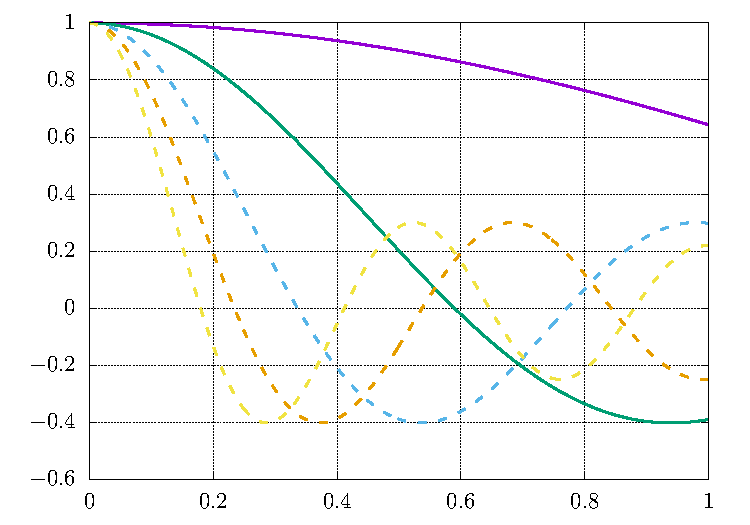
\includegraphics[width=.5\textwidth]{Relatório/Figuras/SingularProblem.pdf}
    \caption{Autofunções (normalizadas) para o problema de Sturm-Liouville
    \eqref{eq:singproblem}.}
    \label{fig:singproblem}
\end{figure}
%
\subsection{Bernoulli\footnote{Este Bernoulli é Daniel, que não é o mesmo Bernoulli
da catenária, Jakob} e outra corda pendurada}
%
Como última aplicação, vamos encontrar, numericamente, os modos normais
de uma corda homogênea pendurada por uma de suas pontas. A dedução da equação
e sua solução podem ser encontradas no Apêndice \ref{ap:cordaproblem}.

O PVC a ser satisfeito pela parte espacial da solução deste problema é dado por
%
\begin{equation}
\label{eq:cordaproblem}
    \left\{
        \begin{array}{l}
            -(gxX')' = \lambda X, \, 0 < x < 1 \\ 
            |X(0)| < \infty, \, X(1) = 0,
        \end{array}
    \right.
\end{equation}
%
sendo $g = 9.8$m/s$^2$ a atração gravitacional. Este é um problema singular como
o estudado na Seção \ref{subsec:singulares}, e podemos resolvê-lo de maneira inteiramente
análoga. Os resultados obtidos são mostrados na Tabela \ref{tab:cordaproblem}
e na Figura \ref{fig:cordaproblem}.
%
\begin{table}[H]
    \centering
    \caption{Intervalos iniciais e autovalores encontrados para o PVC \eqref{eq:cordaproblem}.}
    \begin{tabular}{cc|cc|c}
        % \hline
        \multicolumn{2}{c}{Intervalo inicial} & \multicolumn{2}{c}{Autovalor encontrado} & \\
        \hline
        $a$ & $b$ & $n$ & $\lambda_n$ & \# iterações \\
        \hline
        $1$ & $20$ & $1$ & $14.168845105916262$ & $28$ \\
        $50$ & $80$ & $2$ & $74.656355008482933$ & $27$ \\
        $150$ & $200$ & $3$ & $183.48639830946922$ & $26$ \\
        $200$ & $350$ & $4$ & $340.69997835904360$ & $28$ \\
        $350$ & $800$ & $5$ & $546.32480936124921$ & $29$ \\
        \hline
    \end{tabular}
    \label{tab:cordaproblem}
\end{table}
%
Na Figura \ref{fig:cordaproblem}, o eixo vertical representa a variável $x$
e o ponto $(0,1)$ do gráfico representa o ponto pelo qual a corda está pendurada.
Ademais, os pontos do tipo $(0,\nu)$ nas curvas representadas são os nós
de cada modo normal: o primeiro modo tem apenas o nó $(0,1)$, o segundo modo tem um
nó em $\approx(0,0.2)$ e outro em $(0,1)$, etc.
%
\begin{figure}[H]
    \centering
    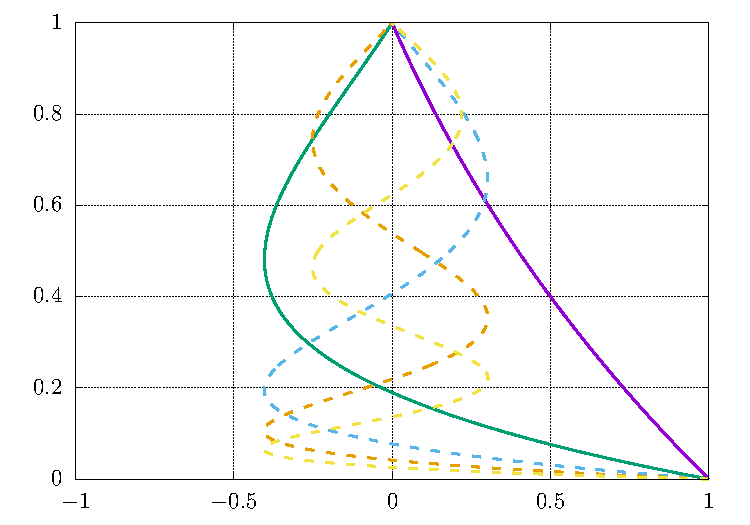
\includegraphics[width=.5\textwidth]{Relatório/Figuras/CordaProblem.pdf}
    \caption{Primeiros 5 modos normais para uma corda pendurada de comprimento 1
    com densidade constante $\rho_0 = 1$.}
    \label{fig:cordaproblem}
\end{figure}
%

% \begin{acknowledgments}
% We thank\dots
% \end{acknowledgments}

% \newpage
\nocite{*}
% \bibliographystyle{apalike}
\bibliographystyle{siam}
% \bibliographystyle{alpha}
\bibliography{referencias}

\appendix

%
\section{A equação da corda pendurada}\label{ap:cordaproblem}
%
Em 1732, Daniel Bernoulli determinou os modos normais de uma corda pendurada
por uma de suas extremidades, utilizando, pela primeira vez, as funções de Bessel
\cite[p.~349]{Sturm-Liouville}.
A corda é modelada como unidimensional e contínua, pendurada verticalmente, com
densidade linear variável e sofrendo deslocamentos transversais de pequena magnitude.
Uma das extremidades está fixa e a outra está livre.

As nossas hipóteses fundamentais são:
%
\begin{itemize}
    \item a corda tem comprimento $\ell$;
    \item apenas a força da gravidade $\mathbf{g}$ e forças de tensão $\mathbf{T}$
    agem na corda;
    \item a aceleração da gravidade é constante;
    \item a tensão atuando em uma dada seção transversal da corda é devida à porção
    de corda abaixo da seção e é tangente à corda.
\end{itemize}
%
Nosso sistema de eixos é definido com o sentido positivo do eixo $x$
direcionado para cima e origem na extremidade livre da corda em repouso.
Seja $\mathbf{R} = x\mathbf{i} + u(x,t)\mathbf{j}$ o vetor posição do ponto
da corda no instante $t$ que ocuparia a posição $x$ no repouso.
Seja $\rho_0(x)$ a densidade linear da corda em equilíbrio e $\rho(x,t)$
a densidade da corda no ponto $x$ e no instante $t$. Denote por $s = s(x,t)$
o comprimento de arco ao longo da corda.

Se $C$ é um segmento da corda que seria $[a,b]$ no repouso, então a conservação
de massa nos diz que
%
\[
    \int_a^b \rho_0(x) \diff x = \int_C \rho \diff s = \int_a^b \rho(x,t)|\mathbf{R}_x| \diff x,
\]
%
ou seja, $\rho_0(x) = \rho(x,t)|\mathbf{R}_x|, \, \forall t$ pois $a$ e $b$ são arbitrários.
Agora, o equilíbrio das forças nos diz que
%
\begin{align*}
    \frac{\diff}{\diff t} \int_C \rho \mathbf{R}_t \diff s 
    &= \mathbf{T}(a,t) - \mathbf{T}(b,t) + \int_C \rho\mathbf{g} \diff s \\
    \frac{\diff}{\diff t} \int_a^b \rho(x,t)\mathbf{R}_t |\mathbf{R}_x| \diff x 
    &= -\int_a^b \mathbf{T}(x,t) \diff x + \int_a^b \rho(x,t)\mathbf{g}|\mathbf{R}_x| \diff x \\
    \frac{\diff}{\diff t}\int_a^b \rho_0(x) \mathbf{R}_t \diff x
    &= -\int_a^b \mathbf{T}(x,t) \diff x + \int_a^b \rho_0(x)\mathbf{g} \diff x \\
    \int_a^b \rho_0(x) \mathbf{R}_{tt} \diff x
    &= -\int_a^b \mathbf{T}(x,t) \diff x + \int_a^b \rho_0(x)\mathbf{g} \diff x.
\end{align*}
%
Novamente, como $a$ e $b$ são arbitrários, segue que
%
\[
    \rho_0(x)\mathbf{R}_{tt} = -\mathbf{T}_x(x,t) + \rho_0(x)\mathbf{g}
\]
%
é a equação diferencial que descreve o movimento da corda. Escrevendo-a em coordenadas,
obtemos
%
\begin{align*}
    \rho_0(x) u_{tt}\mathbf{j}
    &= -\frac{\partial\mathbf{T}}{\partial x} - \rho_0(x)g\mathbf{i} \\
    &= -\frac{\partial}{\partial x}\left( -\frac{T}{|\mathbf{R}_x|}\mathbf{R}_x \right)
    - \rho_0(x)g\mathbf{i} \\
    &= -\frac{\partial}{\partial x}\left( -\frac{T}{|\mathbf{R}_x|}(\mathbf{i} + u_x\mathbf{j})
    \right)
    - \rho_0(x)g\mathbf{i},
\end{align*}
%
ou seja,
%
\[
    \left( \frac{\partial}{\partial x}\left( \frac{T}{|\mathbf{R}_x|} \right)
    - \rho_0(x)g \right)\mathbf{i} + 
    \left( \frac{\partial}{\partial x}\left( \frac{T}{|\mathbf{R}_x|}u_x \right)
    - \rho_0(x)u_{tt} \right)\mathbf{j}
    = \mathbf{0}.
\]
%
Portanto,
%
\begin{align*}
    \frac{\partial}{\partial x}\left( \frac{T}{|\mathbf{R}_x|} \right)
    &= \rho_0(x)g \\
    \frac{\partial}{\partial x}\left( \frac{T}{|\mathbf{R}_x|}u_x \right)
    &= \rho_0(x)u_{tt}.
\end{align*}
%
Como $T(0,t) = 0$, integrando a primeira equação de $0$ a $x$ nos dá
%
\[
    \frac{T}{|\mathbf{R}_x|} = \int_0^x \rho_0(\tau) g \diff\tau
\]
%
e a segunda nos dá
%
\[
    \rho_0(x)u_{tt} = \left( u_x\int_0^x \rho_0(\tau) g \diff\tau \right)_x,
\]
%
que é a equação da onda para as oscilações transversais da corda $u(x,t)$.
Considerando as hipóteses iniciais, o PVIC para esta corda é
%
\[
    \left\{
        \begin{array}{l}
            \rho_0(x) u_{tt} = (p(x)u_x)_x, \, 0 < x < \ell, \, t > 0 \\ 
            |u(0,t)| < \infty, \, u(\ell, t) = 0, \, t\geq 0 \\ 
            u(x,0) = f(x), \, u_t(x,0) = v(x), \, 0 \leq x \leq \ell,
        \end{array}
    \right.
\]
%
sendo $f(x)$ o formato inicial da corda, $v(x)$ o perfil de velocidade inicial da corda
e
%
\[
    p(x) = g\int_0^x \rho_0(\tau) g \diff\tau.
\]
%
Como $p(0) = 0$, a equação diferencial é singular. Isto faz com que as equações
tenham soluções limitadas e ilimitadas. Para que uma solução seja fisicamente
razoável, precisamos que a solução seja limitada, e daí vem a condição de contorno
$|u(0,t)| < \infty$, que diz que o deslocamento é limitado para todo $t$.

Para encontrar os modos normais, propomos uma solução separada da forma
%
\[
    u(x,t) = T(t)X(x).
\]
%
Uma tal solução satisfaz a EDP se, e só se,
%
\begin{align*}
    \rho_0(x)T_{tt}X = T(p(x)X')' \iff
    \frac{T_{tt}}{T} = \frac{(p(x) X')'}{\rho_0(x) X} = -\lambda.
\end{align*}
%
Acrescentando as condições de contorno, temos
%
\[
    \left\{
        \begin{array}{l}
            -(p(x)X')' = \lambda\rho_0(x)X, \, 0 < x < \ell \\ 
            |X(0)| < \infty, \, X(\ell) = 0
        \end{array}
    \right.
\]
%
e $T_{tt} + \lambda T = 0$. Em particular, se $\rho_0(x) \equiv 1$ e $\ell = 1$, obtemos
%
\[
    \left\{
        \begin{array}{l}
            -(gxX')' = \lambda X, \, 0 < x < 1 \\ 
            |X(0)| < \infty, \, X(1) = 0,
        \end{array}
    \right.
\]
%
que nada mais é do que \eqref{eq:cordaproblem}.

%
\section{Códigos utilizados}
%
Os códigos escritos para este projeto podem ser encontrados 
\href{https://github.com/CaioTomas/Trabalho-final----IMCEDO}{neste link}.

\end{document}